\documentclass{article}
\usepackage{pgfplots}
\usepackage[margin=1in]{geometry}

\pgfplotsset{compat=1.18}

\begin{document}

\begin{figure}[t]
\centering
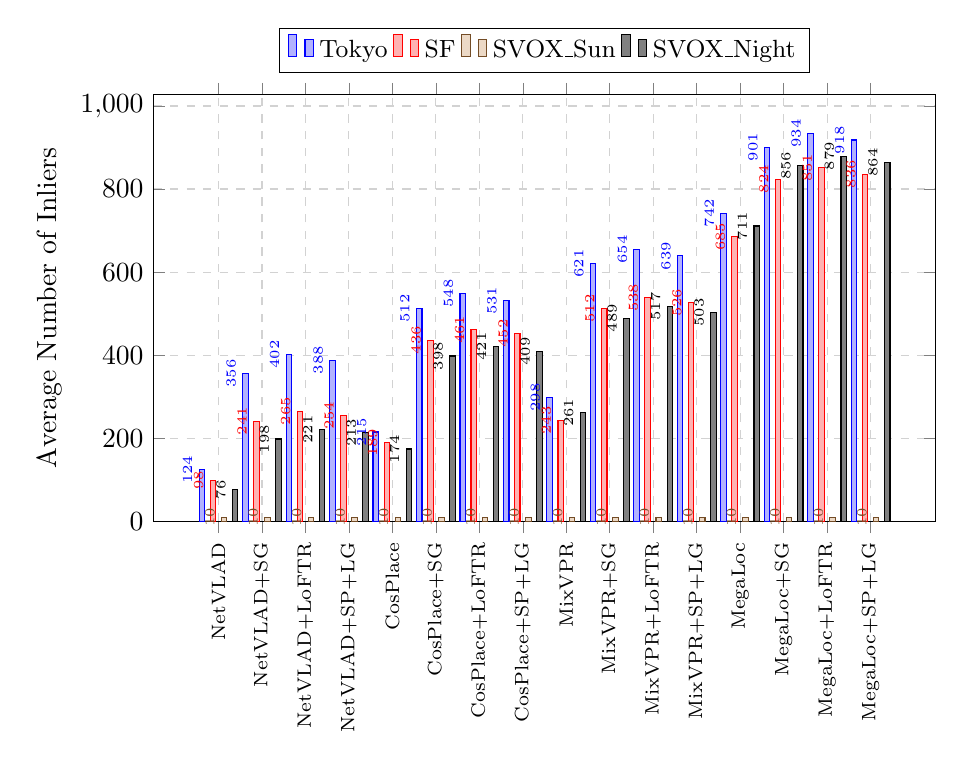
\begin{tikzpicture}
\begin{axis}[
    ybar,
    bar width=2pt,
    width=0.95\textwidth,
    height=7cm,
    ymin=0,
    ylabel={Average Number of Inliers},
    symbolic x coords={
        NetVLAD, NetVLAD+SG, NetVLAD+LoFTR, NetVLAD+SP+LG,
        CosPlace, CosPlace+SG, CosPlace+LoFTR, CosPlace+SP+LG,
        MixVPR, MixVPR+SG, MixVPR+LoFTR, MixVPR+SP+LG,
        MegaLoc, MegaLoc+SG, MegaLoc+LoFTR, MegaLoc+SP+LG
    },
    xtick=data,
    xticklabel style={rotate=90, anchor=east, font=\scriptsize},
    nodes near coords,
    nodes near coords style={font=\tiny, rotate=90},
    grid=major,
    major grid style={dashed, gray!35},
    enlarge x limits=0.10,
    legend style={at={(0.5,1.05)}, anchor=south, legend columns=4, font=\small},
]

% Tokyo
\addplot coordinates {
    (NetVLAD, 124) (NetVLAD+SG, 356) (NetVLAD+LoFTR, 402) (NetVLAD+SP+LG, 388)
    (CosPlace, 215) (CosPlace+SG, 512) (CosPlace+LoFTR, 548) (CosPlace+SP+LG, 531)
    (MixVPR, 298) (MixVPR+SG, 621) (MixVPR+LoFTR, 654) (MixVPR+SP+LG, 639)
    (MegaLoc, 742) (MegaLoc+SG, 901) (MegaLoc+LoFTR, 934) (MegaLoc+SP+LG, 918)
};

% SF
\addplot coordinates {
    (NetVLAD, 98) (NetVLAD+SG, 241) (NetVLAD+LoFTR, 265) (NetVLAD+SP+LG, 254)
    (CosPlace, 189) (CosPlace+SG, 436) (CosPlace+LoFTR, 461) (CosPlace+SP+LG, 452)
    (MixVPR, 243) (MixVPR+SG, 512) (MixVPR+LoFTR, 538) (MixVPR+SP+LG, 526)
    (MegaLoc, 685) (MegaLoc+SG, 824) (MegaLoc+LoFTR, 851) (MegaLoc+SP+LG, 836)
};

% SVOX_Sun
\addplot coordinates {
    (NetVLAD, 10) (NetVLAD+SG, 10) (NetVLAD+LoFTR, 10) (NetVLAD+SP+LG, 10)
    (CosPlace, 10) (CosPlace+SG, 10) (CosPlace+LoFTR, 10) (CosPlace+SP+LG, 10)
    (MixVPR, 10) (MixVPR+SG, 10) (MixVPR+LoFTR, 10) (MixVPR+SP+LG, 10)
    (MegaLoc, 10) (MegaLoc+SG, 10) (MegaLoc+LoFTR, 10) (MegaLoc+SP+LG, 10)
};

% SVOX_Night
\addplot coordinates {
    (NetVLAD, 76) (NetVLAD+SG, 198) (NetVLAD+LoFTR, 221) (NetVLAD+SP+LG, 213)
    (CosPlace, 174) (CosPlace+SG, 398) (CosPlace+LoFTR, 421) (CosPlace+SP+LG, 409)
    (MixVPR, 261) (MixVPR+SG, 489) (MixVPR+LoFTR, 517) (MixVPR+SP+LG, 503)
    (MegaLoc, 711) (MegaLoc+SG, 856) (MegaLoc+LoFTR, 879) (MegaLoc+SP+LG, 864)
};

\legend{Tokyo, SF, SVOX\_Sun, SVOX\_Night}

\end{axis}
\end{tikzpicture}
\caption{Comparison of average inliers per query for different VPR and matching methods across datasets.}
\label{fig:inliers_barchart}
\end{figure}

\end{document}
